The PMT box (figure ) comprehends two PMTs used to trigger the \laserii~acquisition in the LASER mode. It houses two electronic boards :
\begin{itemize}

\item LicPMT (Fig. \ref{fig:laslicpmt}) : this module is used to set the high voltage to the twp PMTs located in the box. It provides measurements of temperature and humidity inside of the optics box and is used to manage the interlock chain that preventes users from flashing the \laser~when the optics box is open. LicPMT is also implied in the configuration and the control of the laser pump (slow control part) and is used to switch the \laser~pump (power supply relay) on. 



\begin{figure}[htbp]
\centering
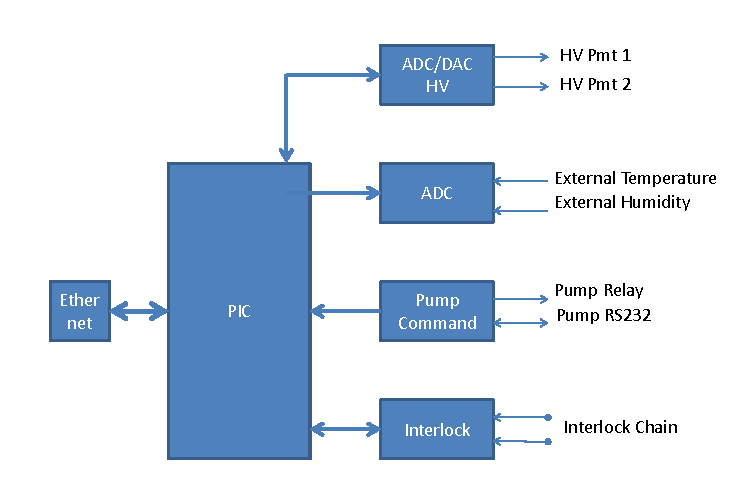
\includegraphics[height=5cm]{figures/licpmt_scheme.pdf}
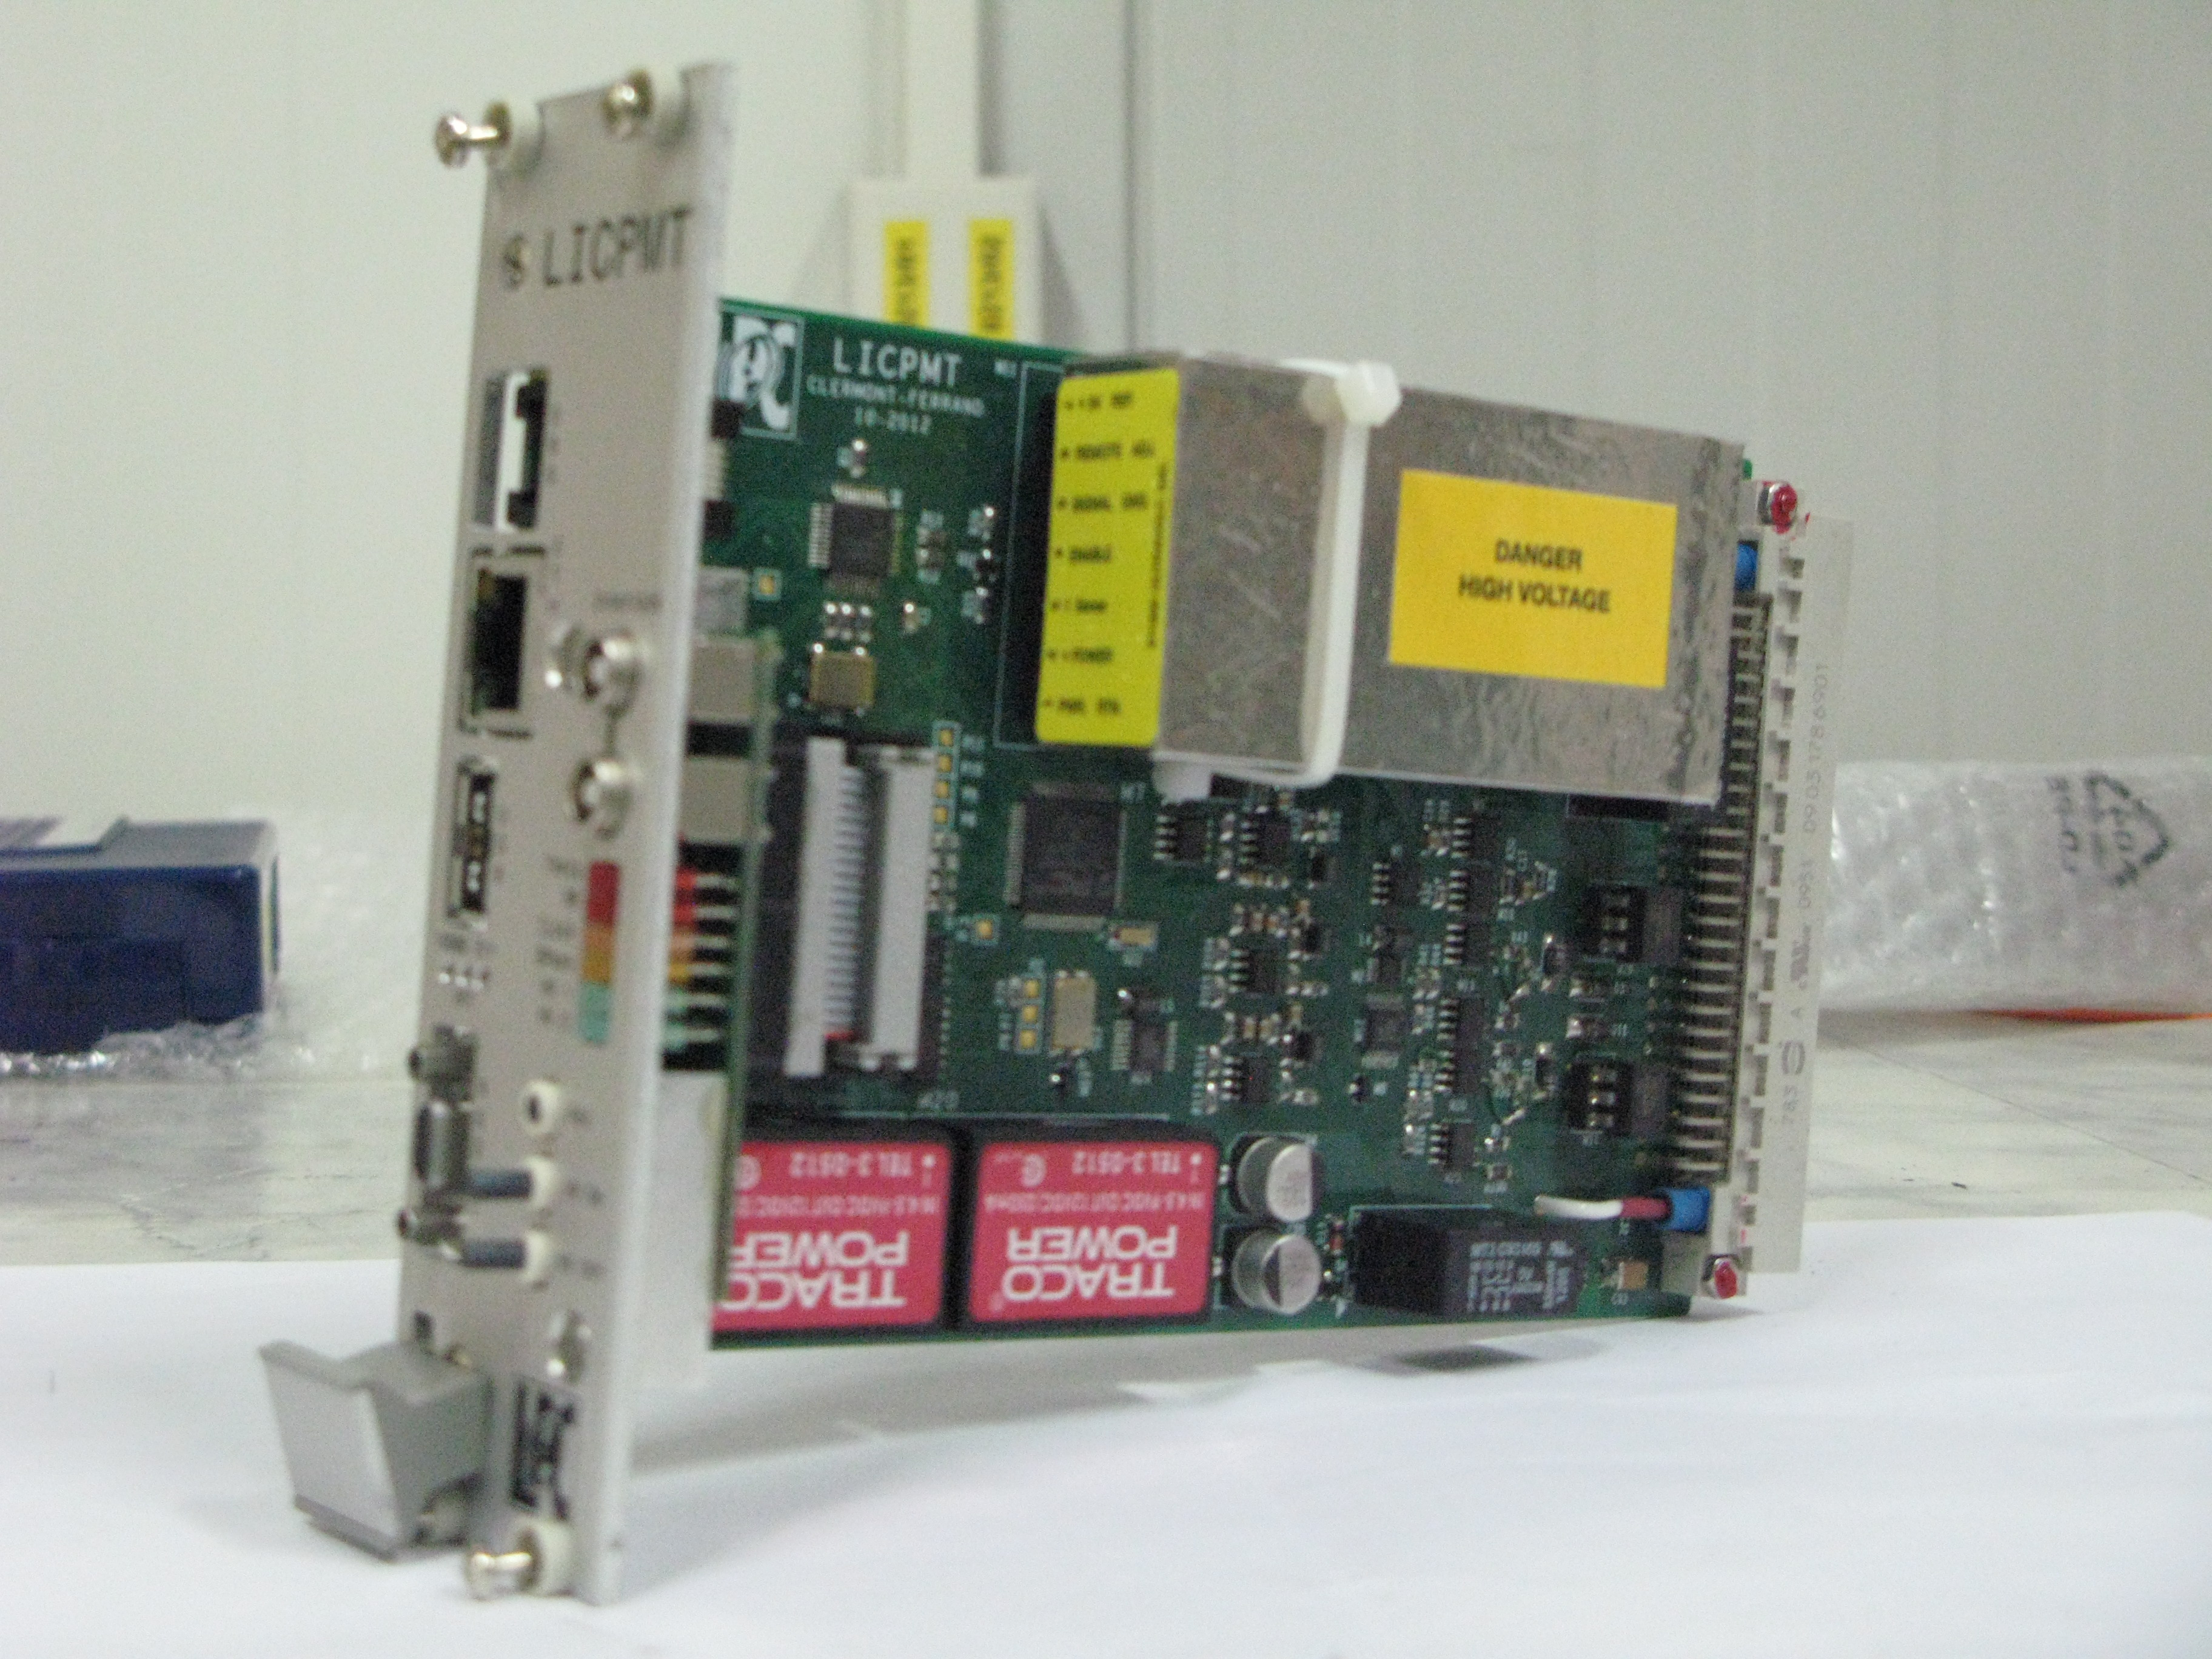
\includegraphics[height=5cm]{figures/licpmt.JPG}
\caption{View of the LicPMT card}\label{fig:laslicpmt}
\end{figure}

\item LicMot (Fig. \ref{fig:laslicmot}) : this module is used to manage the shutter and the two filter wheels (one at a time). The choice between the two wheels is carried out as follows : the homemade wheel is activated when the wheel position board is connected to the LicMot card. Otherwise, the Newport wheel is in use.

\begin{figure}[htbp]
\centering
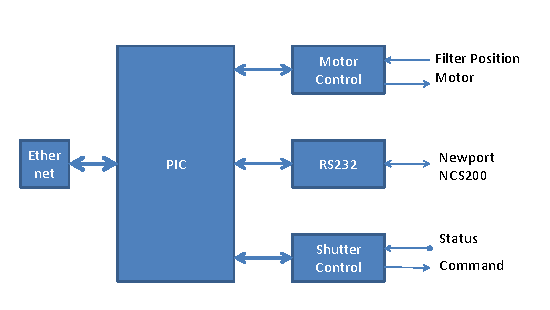
\includegraphics[height=5cm]{figures/licmot_scheme.pdf}
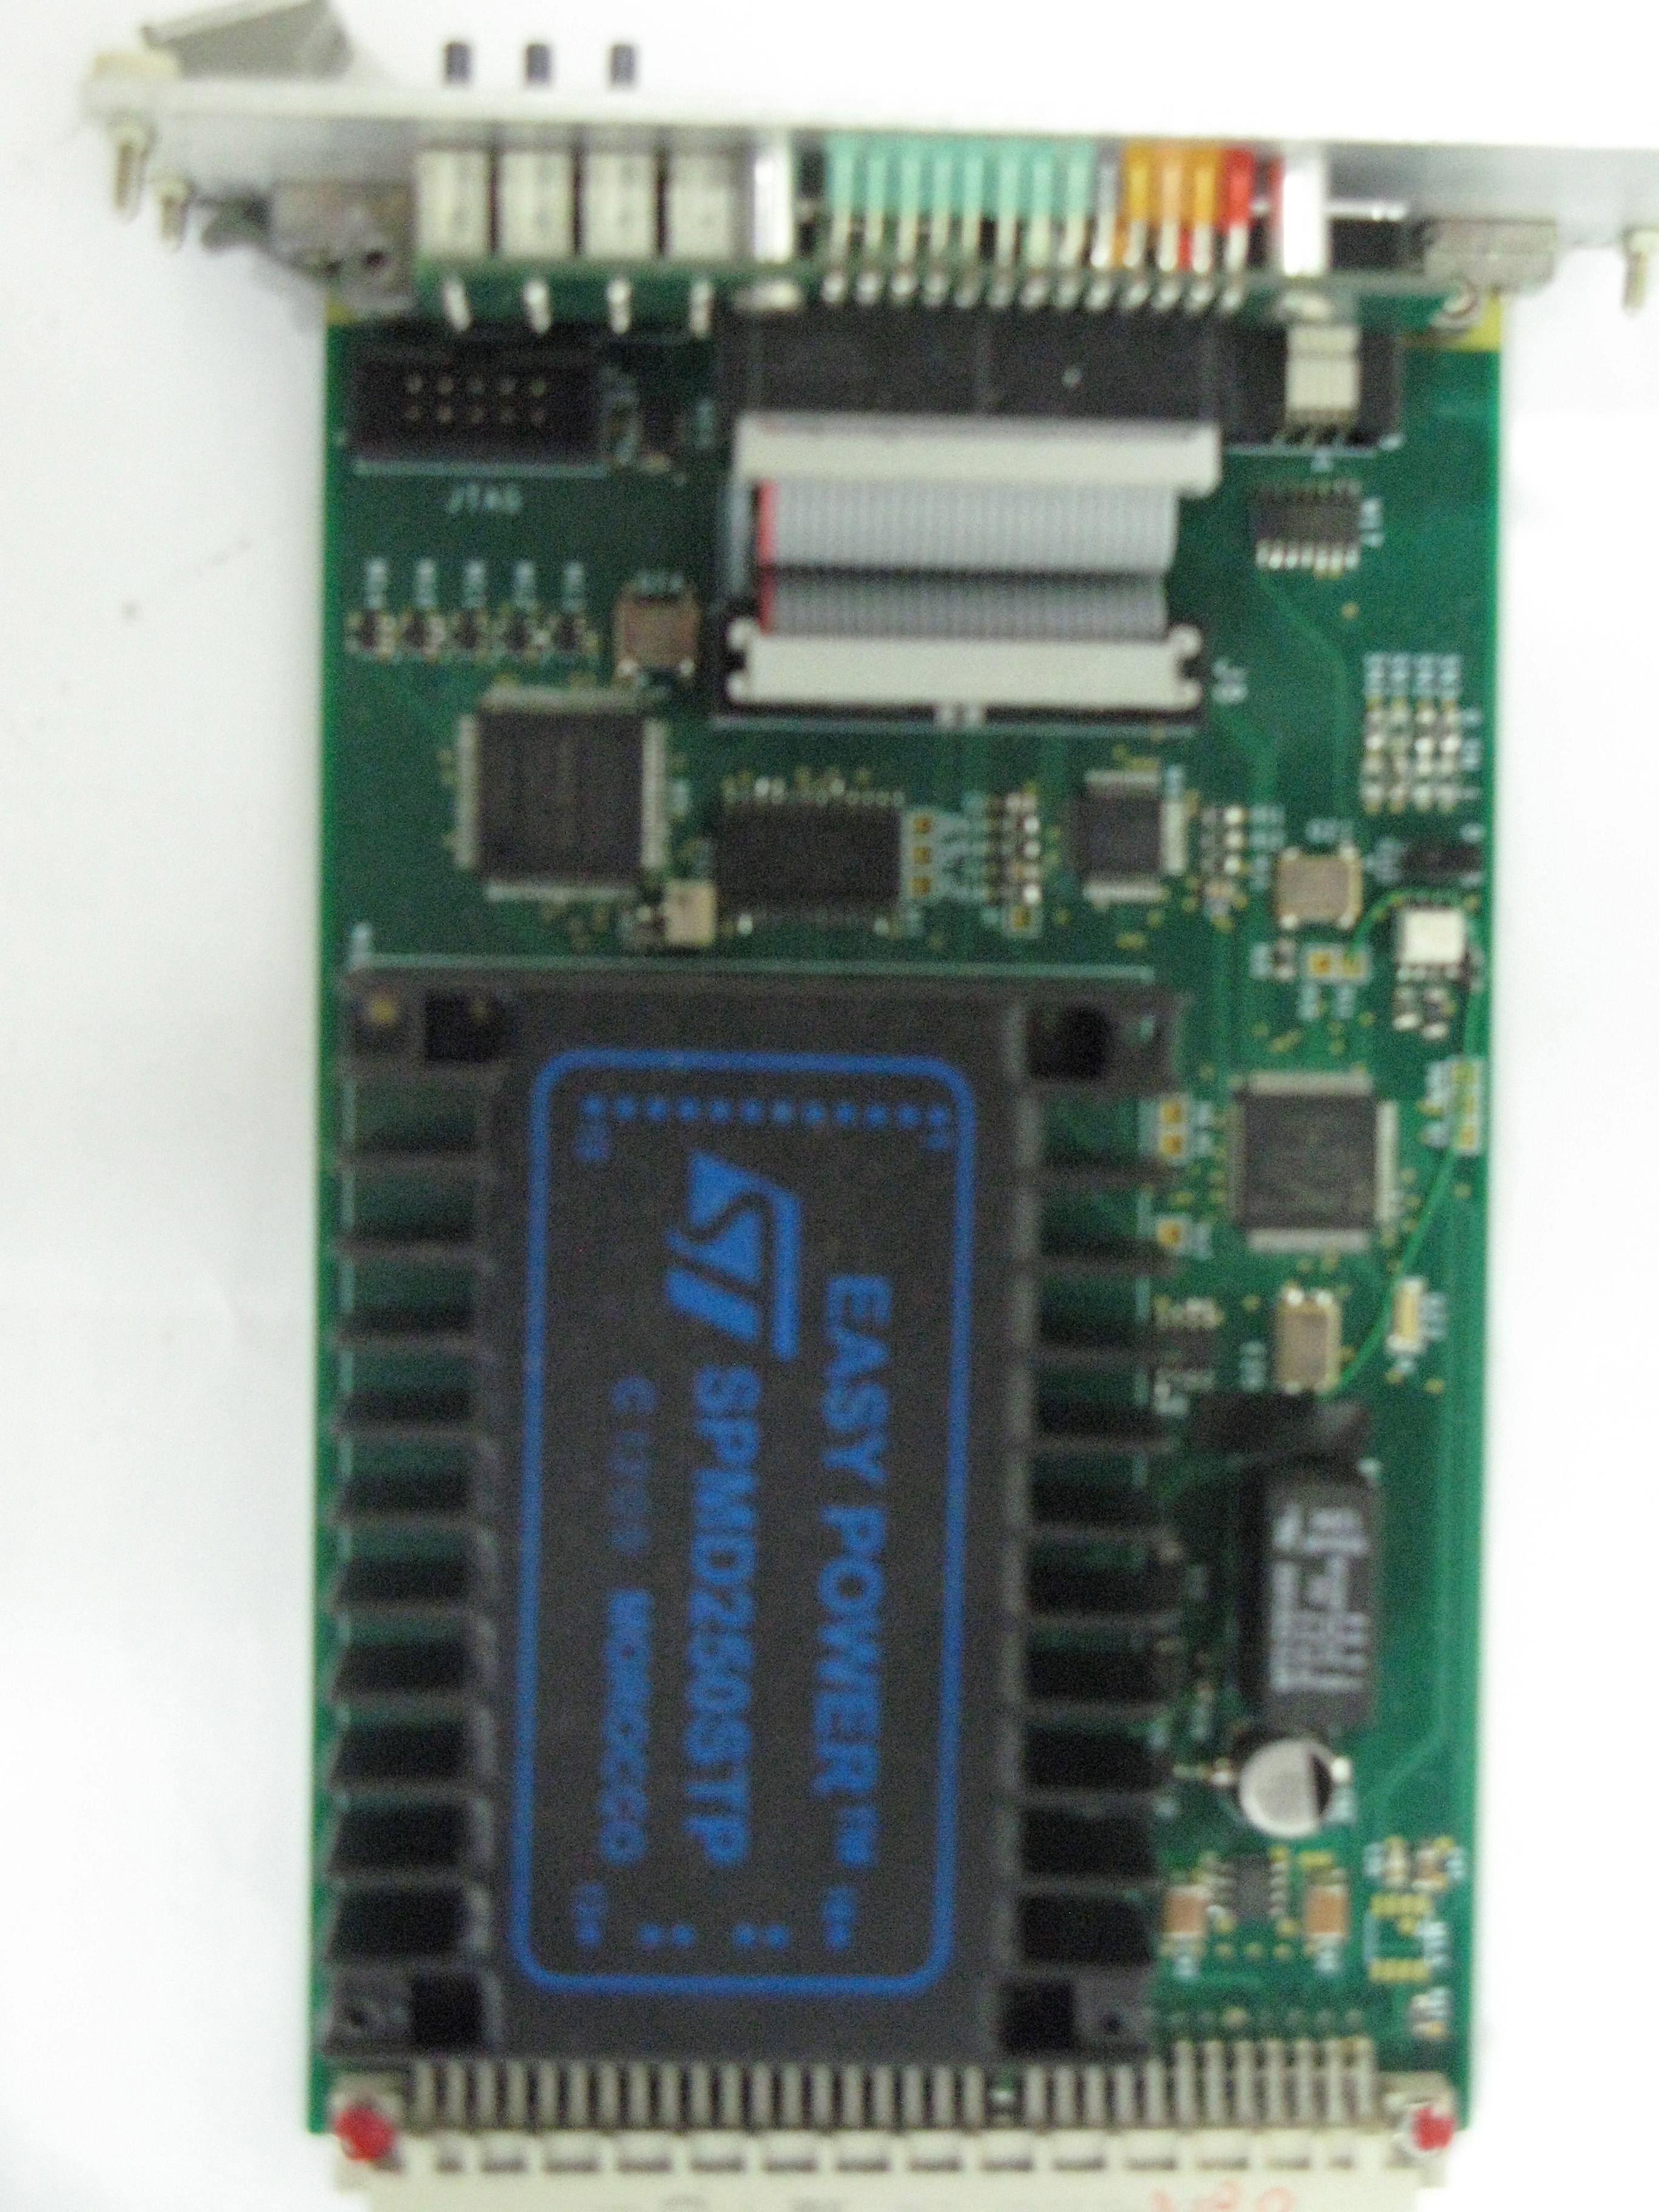
\includegraphics[height=5cm]{figures/licmot.JPG}
\caption{View of the LicMot card}\label{fig:laslicmot}
\end{figure}

\end{itemize}
